\documentclass[landscape,a0paper,fontscale=0.285]{baposter} % Adjust the font scale/size here

\usepackage{graphicx} % Required for including images
\graphicspath{{figures/}} % Directory in which figures are stored

\usepackage{amsmath} % For typesetting math
\usepackage{amssymb} % Adds new symbols to be used in math mode

\usepackage{booktabs} % Top and bottom rules for tables
\usepackage{enumitem} % Used to reduce itemize/enumerate spacing
\usepackage{palatino} % Use the Palatino font
\usepackage[font=small,labelfont=bf]{caption} % Required for specifying captions to tables and figures

\usepackage{multicol} % Required for multiple columns
\setlength{\columnsep}{1.5em} % Slightly increase the space between columns
\setlength{\columnseprule}{0mm} % No horizontal rule between columns

\usepackage{tikz} % Required for flow chart
\usetikzlibrary{shapes,arrows} % Tikz libraries required for the flow chart in the template

\usepackage{url}

\newcommand{\compresslist}{ % Define a command to reduce spacing within itemize/enumerate environments, this is used right after \begin{itemize} or \begin{enumerate}
\setlength{\itemsep}{1pt}
\setlength{\parskip}{0pt}
\setlength{\parsep}{0pt}
}

\definecolor{lightblue}{rgb}{0.145,0.6666,1} % Defines the color used for content box headers

\begin{document}

\begin{poster}
{
headerborder=closed, % Adds a border around the header of content boxes
colspacing=1em, % Column spacing
bgColorOne=white, % Background color for the gradient on the left side of the poster
bgColorTwo=white, % Background color for the gradient on the right side of the poster
borderColor=lightblue, % Border color
headerColorOne=black, % Background color for the header in the content boxes (left side)
headerColorTwo=lightblue, % Background color for the header in the content boxes (right side)
headerFontColor=white, % Text color for the header text in the content boxes
boxColorOne=white, % Background color of the content boxes
textborder=roundedleft, % Format of the border around content boxes, can be: none, bars, coils, triangles, rectangle, rounded, roundedsmall, roundedright or faded
eyecatcher=true, % Set to false for ignoring the left logo in the title and move the title left
headerheight=0.1\textheight, % Height of the header
headershape=roundedright, % Specify the rounded corner in the content box headers, can be: rectangle, small-rounded, roundedright, roundedleft or rounded
headerfont=\Large\bf\textsc, % Large, bold and sans serif font in the headers of content boxes
%textfont={\setlength{\parindent}{1.5em}}, % Uncomment for paragraph indentation
linewidth=2pt % Width of the border lines around content boxes
}
%----------------------------------------------------------------------------------------
%	TITLE SECTION
%----------------------------------------------------------------------------------------
%
{
\includegraphics[height=5em]{RIT_tiger.png}} % First university/lab logo on the left
{\bf\textsc{Multi-Messenger Astrophysics Parameter Estimation for GW
and EM data channels}\vspace{-0.1em}} % Poster title
{\textsc{ Benjamin Champion, Ofek Birnholtz \& Richard O'Shaughnessy \\
	\hspace{12pt} Center for Computational Relativity and Gravitation, Rochester Institute of Technology}}
{
\includegraphics[height=5em]{ccrg_logo.png}} % Second university/lab logo on the right

%----------------------------------------------------------------------------------------
%	Overview
%----------------------------------------------------------------------------------------

\headerbox{Overview}{name=objectives,column=0,span=2,row=0}{

Donec non nisl a \textbf{arcu consequat} varius. Sed suscipit cursus luctus. Nulla sit amet elit augue. Curabitur scelerisque mollis dolor, quis blandit lorem condimentum at. Pellentesque sed nibh vel \textbf{dolor} sagittis semper.

\begin{enumerate}\compresslist
\item Feugiat vitae elit
\item bibendum ante sed lacinia eros in
\item Curabitur scelerisque arcu consequat varius
\item Dapibus nulla id purus consectetur
\item Fringilla integer
\end{enumerate}

\vspace{0.3em} % When there are two boxes, some whitespace may need to be added if the one on the right has more content
}


%	REFERENCES
%----------------------------------------------------------------------------------------

\headerbox{References}{name=references,column=0,span=3,above=bottom}{

\begin{multicols}{2}

\renewcommand{\section}[2]{\vskip 0.05em} % Get rid of the default "References" section title
\nocite{*} % Insert publications even if they are not cited in the poster
\small{ % Reduce the font size in this block
\bibliographystyle{unsrt}
\bibliography{poster_bibliography}
}

\end{multicols}

}
%----------------------------------------------------------------------------------------



%----------------------------------------------------------------------------------------
%	Code Design
%----------------------------------------------------------------------------------------

\headerbox{Code Design}{name=codedesign,below=objectives=2,span=2,above=references}%,bottomaligned=conclusion}
{

\begin{multicols}{2}
\begin{center}
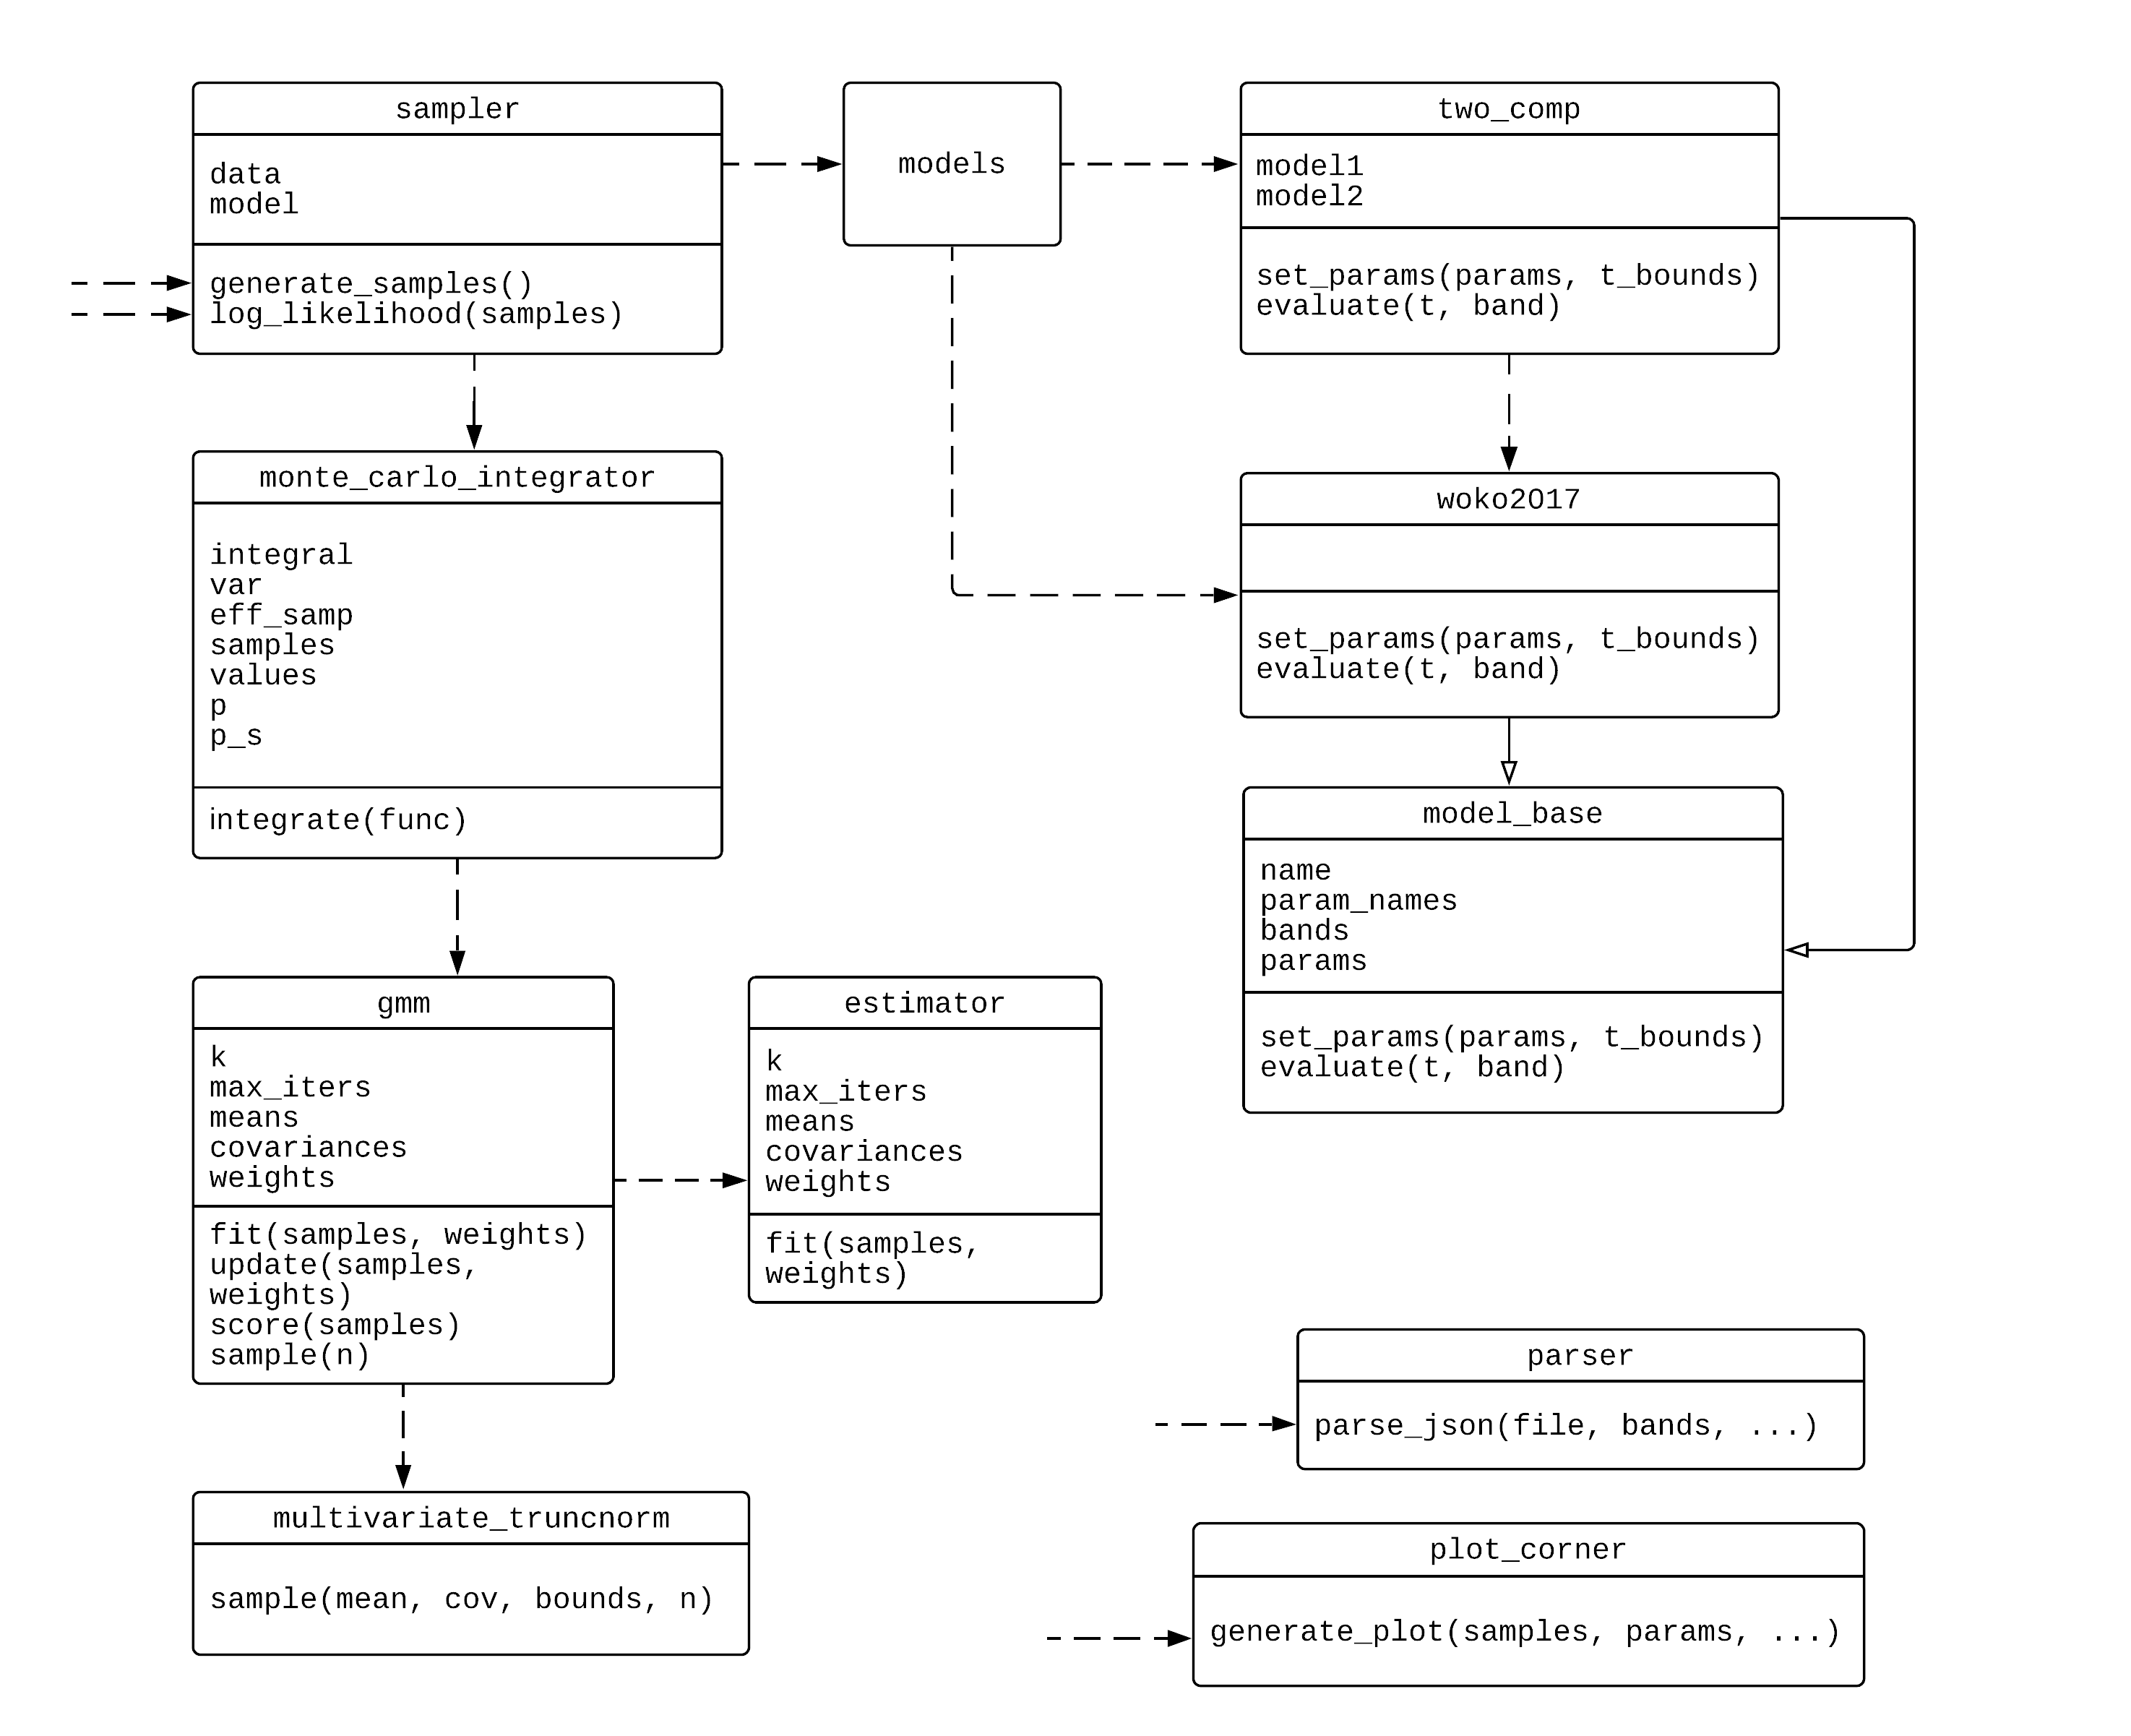
\includegraphics[width=1.83\linewidth]{UML2}
\captionof{figure}{code}
\end{center}

\end{multicols}

\vspace{1em}

}
%----------------------------------------------------------------------------------------


%----------------------------------------------------------------------------------------
%	Recovery Plots 1
%----------------------------------------------------------------------------------------

\headerbox{Recovery of Injection}{name=recovery,column=2,row=0}
{ % This block's bottom aligns with the bottom of the conclusion block

\begin{center}
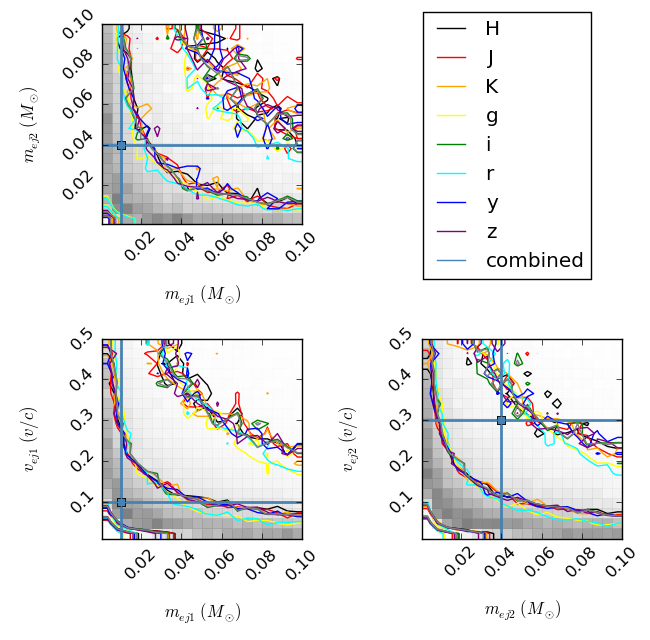
\includegraphics[width=1\linewidth]{syn_combined_corner_poster.png}
\captionof{figure}{Recovery of injection across bands}
\end{center}

}

%----------------------------------------------------------------------------------------
%	Light Curves 1
%----------------------------------------------------------------------------------------

\headerbox{Mock Light Curves}{name=lightcurves,column=3,row=0,bottomaligned=recovery}
{ % This block's bottom aligns with the bottom of the conclusion block

\begin{center}
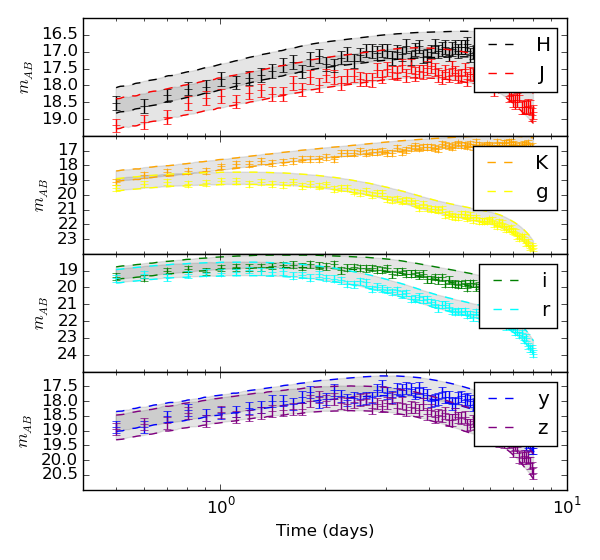
\includegraphics[width=1\linewidth]{lc_synthetic}
\captionof{figure}{Synthetic lightcurves}
\end{center}


}

%----------------------------------------------------------------------------------------

%----------------------------------------------------------------------------------------
%	Recovery Plots 2
%----------------------------------------------------------------------------------------

\headerbox{Recovery of GW170817}{name=recovery2,column=2,below=recovery}
{ % This block's bottom aligns with the bottom of the conclusion block

\begin{center}
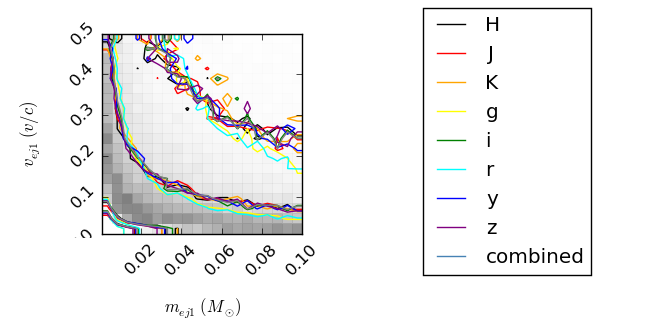
\includegraphics[width=1\linewidth]{real_combined_corner_poster_thin}
\captionof{figure}{Recovery of GW170817 across bands}
\end{center}

}

%----------------------------------------------------------------------------------------
%	Light Curves 2
%----------------------------------------------------------------------------------------

\headerbox{Real Light Curves}{name=lightcurves2,column=3,below=lightcurves,bottomaligned=recovery2}
{ % This block's bottom aligns with the bottom of the conclusion block

\begin{center}
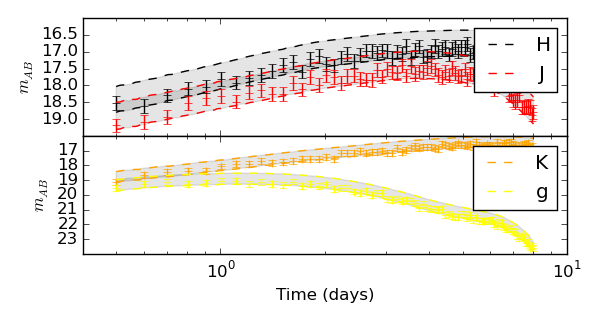
\includegraphics[width=1\linewidth]{lc_real_thin}
\captionof{figure}{GW170817 lightcurves}
\end{center}


}
%----------------------------------------------------------------------------------------


%----------------------------------------------------------------------------------------



%----------------------------------------------------------------------------------------
%	CONCLUSION
%----------------------------------------------------------------------------------------

\headerbox{Conclusion \& Future Research}{name=conclusion,column=2,span=2,row=0,below=recovery2,above=references}{

\begin{multicols}{2}

\begin{itemize}\compresslist
\item Pellentesque eget orci eros. Fusce ultricies, tellus et pellentesque fringilla, ante massa luctus libero, quis tristique purus urna nec nibh. Phasellus fermentum rutrum elementum. Nam quis justo lectus.
\item Vestibulum sem ante, hendrerit a gravida ac, blandit quis magna.
\end{itemize}

\end{multicols}
}
%----------------------------------------------------------------------------------------



%----------------------------------------------------------------------------------------
%	CONTACT INFORMATION
%----------------------------------------------------------------------------------------

\headerbox{Contact Information}{name=contact,column=3,aligned=references,above=bottom}{ % This block is as tall as the references block

\begin{description}\compresslist
\item[Web] https://ccrg.rit.edu/
\item[Email] bwc3252@rit.edu
\item[Phone] +1 (585) 475 5943
\end{description}
}



\end{poster}

\end{document}
